% disc.tex
\chapter{Analyse numérique}

\section{Discrétisation temporelle}

La résolution numérique des équations considérées se fait par la méthode des lignes. Il s'agit de discrétiser dans un premier temps les opérateurs spatiaux pour aboutir à une équations semi-discrétisée. Il ne reste que la dimension temporelle à considérer : il s'agit de la résolution numérique d'une équation aux dérivées ordinaires (EDO). Nous considérons ici des EDO de la forme
\begin{equation}
\dfrac{d q}{dt} = J_{\Delta} (q)
\label{eq:edo}
\end{equation}
avec la condition initiale $q(0)=q_0$. 
Ce choix de méthode est essentiellement pratique. La discrétisation spatiale et la discrétisation temporelle sont séparées, cela facilite le développement de nouvelles méthodes de discrétisations qui peuvent aisément être changées dans le code.

\subsection{Discrétisation de Runge-Kutta d'ordre 4}

Le schéma de résolution temporelle de référence que nous considérons est le schéma de Runge-Kutta d'ordre 4 (RK4). Si nous connaissons l'état de $q$ au temps $t^n = n \Delta t$ (que nous noterons $q^n$) alors nous cherchons à déterminer de façon explicite une valeur approchée de $q$ au temps $t^{n+1} = (n+1) \Delta t$. C'est à dire que nous cherchons $Q$ tel que
\begin{equation}
q^{n+1} = Q(q^n)
\end{equation}
Le schéma de Runge-Kutta d'ordre 4 est l'une des méthodes de Runge-Kutta les plus répandu, il s'écrit suivant l'algorithme \ref{alg:RK4}.

\begin{center}
\begin{minipage}[H]{12cm}
  \begin{algorithm}[H]
    \caption{: RK4}\label{alg:RK4}
    \begin{algorithmic}[1]
    \State $q^0 = q_0$ connu,
    \For{$n=0,1, \ldots$}
             \State  $K^{(1)} = J_{\Delta} \left( q^n \right)$,
             \State  $K^{(2)} = J_{\Delta} \left( q^n + \dfrac{\Delta t}{2} K^{(1)}\right)$,
             \State  $K^{(3)} = J_{\Delta} \left( q^n + \dfrac{\Delta t}{2} K^{(2)}\right)$,
             \State  $K^{(4)} = J_{\Delta} \left( q^n + \Delta t K^{(3)}\right)$,  
             \State  $q^{n+1} = q^n  + \dfrac{\Delta t}{6} \left( K^{(1)} + 2 K^{(2)} + 2 K^{(3)} + K^{(4)} \right)$.
            \EndFor
    \end{algorithmic}
    \end{algorithm}
\end{minipage}
\end{center}

On dit qu'une méthode numérique est consistante \cite{Demailly2016} si
\begin{equation}
q^n - q(n \Delta t) = e^n
\end{equation}
et $e^n \rightarrow 0$ lors que $\Delta t \rightarrow 0$.

Il existe autres méthodes de Runge-Kutta explicites. On pensera par exemples à la méthode d'Euler Explicite ou le schéma de Heun. Il est classique de représenter une méthode de Runge-Kutta par son \textit{tableau de Butcher} :

\begin{table}[htbp]
\begin{center}
\begin{tabular}{c|c}
$b$ & $R$ \\
\hline
    & $c^T$
\end{tabular}
\end{center}
\caption{Tableau de Butcher d'une méthode de Runge-Kutta.}
\label{tab:butcher}
\end{table}

où $R$ est une matrice, $b$ et $c$ sont des vecteurs. Par exemple, le tableau de Butcher de la méthode de Runge Kutta d'ordre 4 de l'algorithme \ref{alg:RK4} est donné par :

\begin{table}[htbp]
\begin{center}
\begin{tabular}{c|cccc}
$0$   &       &      &      &      \\
$1/2$ & $1/2$ &      &      &      \\
$1/2$ & $0$   & $1/2$&      &      \\
$1$   & $0$   & $0$  & $1$  &      \\  
\hline
      & $1/6$ & $1/3$& $1/3$& $1/6$\\
\end{tabular}
\end{center}
\caption{Tableau de Butcher de la méthode de Runge Kutta d'ordre 4 (algorithme \ref{alg:RK4}).}
\end{table}
Les matrices associées au tableau de Butcher pour RK4 sont
\begin{equation}
R= \begin{bmatrix}
0 & 0 & 0 & 0 \\
1/2& 0& 0 & 0 \\
0 &1/2& 0 & 0 \\
0 & 0 & 1 & 0
\end{bmatrix}
\hspace{1cm}
b=\begin{bmatrix}
0\\1/2\\1/2\\1
\end{bmatrix}
\hspace{1cm}
c=\begin{bmatrix}
1/6\\1/3\\1/3\\1/6
\end{bmatrix}.
\end{equation}

\begin{proposition}
Une méthode de Runge-Kutta est explicite si $R$ est triangulaire inférieure strictement.
\end{proposition}




\subsection{Stabilité}

La \textit{stabilité linéaire} d'un schémas en temps est une notion essentielle associée à un schéma. Cette notion recouvre de nombreux aspects dans la littérature.
Un schéma d'intégration en temps permet de calculer $q^n$ une approximation de $q(n \Delta t)$ à une erreur $e^n$ près :
\begin{equation}
q^n = q(n \Delta t) + e^n.
\label{eq:scheme_erreur}
\end{equation}

La stabilité du schéma est essentielle. Nous distinguons deux principales notions de stabilité :
\begin{enumerate}
\item La \textit{stabilité au sens de Von Neumann} établi une relation de convergence de $q^n$ vers $q(n \Delta t)$ pour tout $1 \leq n \leq N$ lorsque $\Delta t \rightarrow 0$ et $N \rightarrow + \infty$. 
La stabilité de Von Neumann du schéma \eqref{eq:scheme_erreur} se traduit par
\begin{equation}
\exists C >0, \forall n \in \{ 0 , \cdots , N \}, \forall (N, \Delta t) \in \left\lbrace \mathbb{N} \times \mathbb{R}^+ \text{ tels que } N \Delta t = T \right\rbrace, \| q^n \| \leq C.
\end{equation}
Cette propriété traduit le fait que l'erreur doit rester uniformément bordée lorsque l'on raffine la discrétisation. La stabilité au sens de Von Neumann ne permet pas d'assurer la convergence vers la solution de l'équation différentielle lorsque l'on raffine le maillage, il s'agit là de la consistance. Si un schéma est stable et consistant, alors il y a convergence de la solution numérique vers la solution exacte sur un intervalle borné lorsque l'on raffine, il s'agit du théorème de Lax.

\item La \textit{Stabilité asymptotique} se caractérise par le compostement de la solution numérique $q^n$ sur un intervalle non borné à $\Delta t$ fixé. On distingues deux types de stabilités asymptotiques :
\begin{itemize}
\item la suite $(q^n)_{n \in \mathbb{N}}$ est bornée,
\item La suite $q^n \rightarrow 0$ lorsque $n \rightarrow + \infty$.
\end{itemize}
la stabilité asymptotique est liée à l'équation différentielle résolue. En effet si la solution exacte de l'équation résolue tend vers $0$ alors la solution numérique doit tendre vers $0$ aussi. On note cependant que la stabilité asymptotique peut n'être vérifiée que sous une contrainte sur $\Delta t$.
\end{enumerate} 

Nous nous limitons à la notion de \textit{stabilité linéaire asymptotique}, appelée stabilité linéaire. Il s'agit de la stabilité asymptotique appliquée à l'équation de Dahlquist :
\begin{equation}
\left\lbrace 
\begin{array}{rcl}
q' & = & \lambda q \\
q(0) & = & q_0.
\end{array}
\right.
\label{eq:dahlquist}
\end{equation}
avec $\lambda \in \mathbb{C}^- = \{ \lambda_1 + i \lambda_2 \text{ tels que } (\lambda_1, \lambda_2) \in \mathbb{R}^- \times \mathbb{R} \}$. La solution de cette équation est explicitement donnée par 
\begin{equation}
q(t) = e^{\lambda t} q_0
\end{equation}
On remarque immédiatement que $q$ est bornée (par $q_0$) si Re$(\lambda) \leq 0$ et $q(t) \rightarrow 0$ lorsque $t \rightarrow + \infty$ si Re$(\lambda) <0$.

\begin{proposition}
Soit une méthode de Runge-Kutta appliquée à la résolution de l'équation \eqref{eq:dahlquist}. En utilisant les notations du tableau de Butcher \ref{tab:butcher}, on a 
\begin{equation}
q^{n+1} = r(\lambda \Delta t) q^n,
\end{equation}
avec $r$ donné par 
\begin{equation}
r(\theta) = 1 + \theta c^T \cdot \left( (id - \theta R)^{-1} \mathbf{1} \right).
\end{equation}
\end{proposition}

\begin{proof}
Si l'on note $K = [K_1, K_2, ...]^T$, alors $K$ est solution de 
\begin{equation}
K = \lambda q^n +  \lambda \Delta t R K
\end{equation}
donc, $K = (id - \lambda \Delta t R)^{-1} \mathbf{1}$.
De là, il découle que 
\begin{equation}
q^{n+1} = q^n + \theta c^T \cdot \left( (id - \theta R)^{-1} q^n \right).
\end{equation} 
avec $\theta = \lambda \Delta t$. D'où le résultat.
\end{proof}
On note que si la méthode est explicite alors $R$ est nilpotente donc $r$ est polynomiale en $\theta$, 
en particulier, pour la méthode de Runge-Kutta d'ordre 4, on a 
\begin{equation}
r(\theta) = 1 + \theta + \dfrac{\theta^2}{2} + \dfrac{\theta^3}{6} + \dfrac{\theta^4}{24} 
\end{equation}
alors le résultat de stabilité est le suivant :
\begin{proposition}
La méthode de Runge-Kutta d'ordre 4 (RK4) est asymptotiquement stable pour l'équation \eqref{eq:dahlquist} si et seulement si
\begin{equation}
\vert 1 + \theta + \dfrac{\theta^2}{2} + \dfrac{\theta^3}{6} + \dfrac{\theta^4}{24}  \vert \leq 1,
\end{equation}
avec $\theta = \lambda \Delta t$.
\label{prop:stab_rk4}
\end{proposition}
On définit la zone de stabilité de RK4, notée $\mathcal{D}_{RK4}$, par
\begin{equation}
\mathcal{D}_{RK4} = \left\lbrace \theta \in \mathbb{C} \text{ tels que } \vert 1 + \theta + \dfrac{\theta^2}{2} + \dfrac{\theta^3}{6} + \dfrac{\theta^4}{24}  \vert \leq 1 \right\rbrace
\end{equation} 
Dans la figure \ref{fig:stab_area}, on présente les zones de stabilités de différentes méthodes de Runge-Kutta explicites.
\begin{figure}[htbp]
\begin{center}
\includegraphics[scale=0.2]{stabilityarea_color.jpeg}
\end{center}
\caption{Zones de stabilités de différentes méthodes de Runge-Kutta explicites dans le plan complexe. La zone de stabilité de RK4 est délimitée par le trait noir. Les traits vert, bleu et rouge sont respectivement pour des méthodes de Runge-Kutta d'ordre 3, 2 et 1.}
\label{fig:stab_area}
\end{figure}
En particulier, comme détaillé dans \cite{Hundsdorfer2013}, on note que
\begin{equation}
\mathcal{D}_{RK4} \cap i \mathbb{R} = i \left[-2 \sqrt{2},2 \sqrt{2}\right].
\end{equation}

\begin{proposition}
On suppose que $\Delta t = T/(n+1)$ est choisit tel que $|r(\lambda \Delta t ) | \leq 1$ (RK4 est asymprotiquement stable), alors si $q^{n+1}$ est la solution approchée par RK4 de \eqref{eq:dahlquist} et $q(t)$ la solution exacte en $t \in [0,T]$, il existe $C>0$ tel que
\begin{equation}
| e^{n+1} | = | q^{n+1} - q(t^{n+1}) | \leq C T \Delta t^4 \max_{0 \leq t \leq T} | q(t) |.
\end{equation}
\label{prop:consistance_rk4}
\end{proposition}

\begin{proof}
Par construction des différents termes, on a
\begin{align*}
e^{n+1} & = r(\lambda \Delta t) q^n - \exp \left( \lambda \Delta t \right) q(t^n) \\
	& = r(\lambda \Delta t) \left( q^n - q(t^n) \right) + \left( r(\lambda \Delta t) - \exp \left( \lambda \Delta t  \right) \right) q(t^n) \\
	& = r(\lambda \Delta t) e^n + \left( r(\lambda \Delta t) - \exp \left( \lambda \Delta t  \right) \right) q(t^n).
\end{align*}
D'où, en prenant la valeur absolue, 
\begin{align*}
|e^{n+1}| & \leq |r(\lambda \Delta t)| |e^n| + C \lambda^5 \Delta t^5 q(t^n) \\
		& \leq  |r(\lambda \Delta t| \left[ |r(\lambda \Delta t)| |e^{n-1}| + C \lambda^5 \Delta t^5 |q(t^{n-1})| \right] + C \lambda^5 \Delta t^5 |q(t^n)| \\
		& \leq |r(\lambda \Delta t)|^2 |e^{n-1}| + C \lambda^5 \Delta t^5 |r(\lambda \Delta t)| |q(t^{n-1})| + C \lambda^5 \Delta t^5 |q(t^n)| \\
		& \leq |r(\lambda \Delta t)|^2 |e^{n-1}| + C \lambda^5 \Delta t^5  |q(t^{n-1})| + C \lambda^5 \Delta t^5 |q(t^n)| \text{ par hyposthèse de stabilité.}
		& \leq \vdots \\
		& \leq |r(\lambda \Delta t)|^{n+1} | e^0 | + (n+1) C \lambda^5 \Delta t^5 \max_{0 \leq t \leq T} |q(t)| \\
		& \leq + (n+1) C \lambda^5 \Delta t^5 \max_{0 \leq t \leq T} |q(t)| \text{ car } e^0 = 0 \\
		& \leq C T \lambda^5 \Delta t^4 \max_{0 \leq t \leq T} |q(t)|.
\end{align*}
\end{proof}




\subsection{Schémas de Runge-Kutta pour les systèmes d'équations différentielles}

La notion de stabilité linéaire appliquée à l'équation de Dahlquist \eqref{eq:dahlquist} est étendue au système d'équations différentielles
\begin{equation}
\left\lbrace
\begin{array}{rcl}
\mathbf{q}' & = & J \mathbf{q} \\
\mathbf{q}(0) & = & \mathbf{q}_0 
\end{array}
\right.
\label{eq:dahlquist_mat}
\end{equation}
où $\mathbf{q} = \begin{bmatrix}
q_1(t) & q_2(t) & \cdots & q_N(t)
\end{bmatrix}^T \in \mathbb{R}^N$.
$q_i$ désigne une fonction de $\mathbb{R}^+$ dans $\mathbb{C}$, $J \in \mathbb{M}_N (\mathbb{C})$ désigne une matrice carré. On se restreint au cas où $J$ est une matrice diagonalisable telle que 
\begin{equation}
\text{Sp}(J) \subset \mathbb{C}^-.
\end{equation}
Cette dernière propriété permet d'assurer que la solution de \eqref{eq:dahlquist_mat} est bornée. Cette solution est donnée par 
\begin{equation}
\mathbf{q}(t) = e^{Jt}\mathbf{q}_0 \text{ avec } t \in \mathbb{R}^+.
\end{equation}
Comme $J$ est diagonalisable, il existe $P \in \mathbb{M}_N(\mathbb{R})$ une matrice de passage et $\Lambda \in \mathbb{M}_N(\mathbb{R})$ matrice diagonale (contenant les valeurs propres de $J$) tels que
\begin{equation}
J = P^{-1} \Lambda P
\end{equation}
De la, il vient que 
\begin{equation}
e^{Jt} = P^{-1}e^{\Lambda t}P,
\end{equation}
donc la solution de \eqref{eq:dahlquist_mat} vérifie l'égalité 
\begin{equation}
\mathbf{q}(t) = e^{Jt}\mathbf{q}_0 = P^{-1}e^{\Lambda t}P\mathbf{q}_0.
\end{equation}

A présent,considérons que l'équation \eqref{eq:dahlquist_mat} est discrétisée via la méthode de Runge Kutta d'ordre 4 de l'algorithme \ref{alg:RK4}. On obtient alors 
\begin{equation}
\mathbf{q}^{n+1} = r(\Delta t J) \mathbf{q}^n
\end{equation}
où $r$ est donné par 
\begin{equation}
r(\theta) = 1 + \theta + \dfrac{\theta^2}{2} + \dfrac{\theta^3}{6} + \dfrac{\theta^4}{24}.
\end{equation}
Comme $J$ est diagonalisable, on a même
\begin{equation}
\mathbf{q}^{n+1} = P^{-1}r(\Delta t \Lambda)P \mathbf{q}^n
\end{equation}
De la, on déduit la relation liant $\mathbf{q}^n$ à la condition initiale $\mathbf{q}_0$ : 
\begin{equation}
\mathbf{q}^n = r(\Delta t J) \mathbf{q}_0 = P^{-1}r(\Delta t \Lambda)P \mathbf{q}_0.
\end{equation}
Le schémas utilisé est dit linéairement stable si $\left( \| \mathbf{q}^n \| \right)_{n \in \mathbb{N}}$ est une suite bornée. Comme $J$ est diagonalisable, cela revient à dire que $| r(\Delta t \lambda) | \leq 1$ avec $\lambda \in $ Sp$(J)$.

\begin{proposition}
Le schéma d'intégration est linéairement stable si
\begin{equation}
\forall \lambda \in \text{Sp}(J), |r(\Delta t \lambda)| \leq 1.
\end{equation}
Ce qui est équivalent à dire
\begin{equation}
\text{Sp}(\Delta t J) \subset \mathcal{D}_{RK4}.
\end{equation}
Comme $r$ est un polynôme, on a même la stabilité linéaire si
\begin{equation}
\rho(r(\Delta t J)) \leq 1
\end{equation}
où $\rho$ désigne le rayon spectrale.
\label{prop:stab_rk4_mat}
\end{proposition}








\section{Equation d'advection en dimension 1}

Dans cette section, on s'intéresse à l'équation de transport
\begin{equation}
\dfrac{\partial u}{\partial t} + c \dfrac{\partial u}{\partial x} = 0
\label{eq:transport_1D}
\end{equation}
pour $x \in [0,L]$, $t>0$ et avec $u(t=0,x)=u_0(x)$. On se place en contexte périodique, de période $L$. On a en particulier $u(t,0)=u(t,L)$ pour tout $t \geq 0$. $c$ est une constante positive. La solution exacte de cette équation est connue et donnée par 
\begin{proposition}
La solution de l'équation \eqref{eq:transport_1D} est donnée par 
\begin{equation}
u(t,x) = u_0(x-ct) = \gsum_{k \in \mathbb{Z}} \exp \left[ i \dfrac{2 \pi k}{L} (x-ct) \right] \hat{u}_0^k
\end{equation}
où $\hat{u}_0^k = \dfrac{1}{\sqrt{L}} \gint_0^L u_0(x) \exp \left[ - i \dfrac{2 \pi k}{L}x \right] dx$ désigne la $ki$ème transformée de Fourier de $u_0$.
\end{proposition}

\begin{proof}
La solution de \eqref{eq:transport_1D} est unique, en effet si $u_1$ et $u_2$ sont solutions (distinctes) de \eqref{eq:transport_1D} alors $w = u_1-u_2$ est une solution $L-$périodique de 
\begin{equation}
\dfrac{\partial w}{\partial t} = - \dfrac{\partial  cw}{\partial x}
\end{equation}
vérifiant $w(t=0,x)=0$ pour tout $x$. En multipliant par $w$ et en intégrant sur $[0,L]$, on obtient l'équation
\begin{equation*}
\dfrac{1}{2} \dfrac{d}{dt} \| w \|_{L^2}^2 = - \gint_{0}^L cw \dfrac{\partial w}{\partial x} = - \dfrac{c}{2} \gint_{0}^L \dfrac{\partial w^2}{\partial x} = 0 \text{ par périodicité de }w.
\end{equation*}
donc $\| w \|_{L^2}^2=\| w_{|t=0} \|_{L^2}^2 = 0$ et $w=0$, d'où l'unicité.

On peut facilement vérifier que $(t,x) \mapsto u_0(x-ct)$ et $(t,x) \mapsto \gsum_{k \in \mathbb{Z}} \exp \left[ i \dfrac{2 \pi k}{L} (x-ct) \right] \hat{u}_0^k$ sont solutions de \eqref{eq:transport_1D}. Par unicité de la solution, on obtient le résultat souhaité.
\end{proof}
Cette solution est une translation périodique de la condition initiale. Dans cette section, nous comparons la solution théorique de \eqref{eq:transport_1D} avec une solution numérique obtenue à l'aide de différents opérateurs ou outils de discrétisations évoqués dans les parties précédentes.









\subsection{Discrétisation}

La discrétisation est effectuée en utilisant la méthode des lignes. Dans un premier temps, il s'agit de discrétiser les opérateurs spatiaux. On aboutit à une EDO que nous résolvons par une méthode de Runge-Kutta. Nous utilisons dans cette partie les notations de la section \ref{sec:notation_1D}.
 
On a vu dans les parties précédentes que $\delta_x^H u^*$ était une bonne approximation de $\partial_x u^*$. On remplace l'opérateur de dérivation spatiale $\partial_x$ par l'opérateur de dérivation hermitien $\delta_{4,x}^H$.
On cherche alors $\mathfrak{u}$ approximation de $u^*$ aux points du maillage et solution de 
\begin{equation}
\left\lbrace
\begin{array}{rcl}
\dfrac{d \mathfrak{u}}{dt} & = & - c \delta_{4,x}^H \mathfrak{u} \\
\mathfrak{u}_{|t=0} & = & u_0^*
\end{array}
\right.
\end{equation}
Si l'on note matriciellement 
\begin{equation}
U = \begin{bmatrix}
\mathfrak{u}_1 \\
\mathfrak{u}_2 \\
\vdots \\
\mathfrak{u}_N
\end{bmatrix} \in \mathbb{R}^N \text{ et } U_0 = \begin{bmatrix}
u_0(x_1) \\
u_0(x_2) \\
\vdots \\
u_0(x_N)
\end{bmatrix} \in \mathbb{R}^N
\end{equation}
les vecteurs contenant les composantes de $\mathfrak{u}$ (chaque composante est dépendante de $t$) et de $u_0^*$, alors $U$ est solution du système d'équations différentielles :
\begin{equation}
\left\lbrace
\begin{array}{rcl}
\dfrac{d U}{dt} & = & - c P^{-1}K U \\
U_{|t=0} & = & U_0
\end{array}
\right. .
\end{equation}
La solution d'un tel système est donnée par 
\begin{equation}
U(t) = \exp\left[ - c P^{-1}K t\right] U_0.
\end{equation}

On a déjà vu dans la proposition \ref{prop:eigen_mat_hermitien} que $P^{-1}K$ est une matrice de $\mathbb{M}_N(\mathbb{R})$ qui admet $N$ valeur propres distinctes. $P^{-1}K$ est diagonalisable, il existe $V$ une matrice de passage et $\Lambda$ une matrice diagonale tels que 
\begin{equation}
P^{-1}K = V \Lambda \bar{V}^T.
\end{equation}
Ces matrices sont données par 
\begin{equation}
\Lambda = \begin{bmatrix}
\lambda_1 &   &   &   &   \\ 
  & \lambda_2 &   & (0) &   \\ 
  &   & \ddots &   &   \\ 
  & (0) &   & \lambda_{N-1} &   \\ 
  &   &   &   & \lambda_N
\end{bmatrix} \text{ et }
V = \begin{bmatrix}
  &   &   &   &   \\ 
\vdots & \vdots  &   & \vdots  & \vdots  \\ 
U^1 & U^2 & \cdots & U^{N-1} & U^N \\ 
\vdots &\vdots &  &\vdots &\vdots \\ 
  &   &   &   &  
\end{bmatrix} 
\label{eq:matrice_diagonalisation}
\end{equation}
où les vecteurs propres $U^k$ vérifiant
\begin{equation}
U^k = \vec_1 ( \mathfrak{u}^k )
\end{equation} 
et les valeurs propres associées $\lambda_k = \dfrac{1}{h}Q_{4}^H(\omega^k)$ sont les valeurs propres de $\delta_{4,x}^H$ données par la proposition \ref{prop:eigen_mat_hermitien}. On déduit directement de ces égalités que 
\begin{equation}
U(t) = V \exp \left[-c \Lambda t \right] \bar{V}^T U_0
\end{equation}
d'où, la solution approchée de \eqref{eq:transport_1D} discrétisée en espace et évaluée en $x_j$ est donnée par 

\begin{equation}
u(x_j, t) \approx U_j ( t ) = \dfrac{1}{N} \gsum_{k=0}^{N-1}  \exp \left[ i \dfrac{2 \pi k}{L} x_j - x \omega_k t \right] \gsum_{l=0}^{N-1} \exp \left[ i \dfrac{2 \pi k}{L} x_l \right] u_0 (x_l)
\end{equation}




\begin{lemme}
Pour tout $\alpha > 0$, $\mathfrak{u}, \mathfrak{v} \in \mathcal{l}^2_{h,per}$, on a
\begin{equation}
\alpha |\mathfrak{u}|_{h,per} + \dfrac{1}{\alpha} |\mathfrak{v}|_{h,per} \geq 2 |(\mathfrak{u},\mathfrak{v})_{h,per}|
\end{equation}
\label{lem:ineg_1}
\end{lemme}

\begin{proof}
On a immédiatement
\begin{equation}
\left( \sqrt{\alpha} |\mathfrak{u}|_{h,per} - \dfrac{1}{\sqrt{\alpha}} |\mathfrak{v}|_{h,per} \right)^2 \geq 0
\end{equation}
donc en développant, on a
\begin{equation}
\alpha |\mathfrak{u}|_{h,per}^2 - 2 |\mathfrak{u}|_{h,per} |\mathfrak{v}|_{h,per} + \dfrac{1}{\alpha} |\mathfrak{v}|_{h,per}^2 \geq 0.
\end{equation}
Ainsi, en utilisant l'inégalité de Cauchy-Schwarz, il vient
\begin{equation}
\alpha |\mathfrak{u}|_{h,per}^2 + \dfrac{1}{\alpha} |\mathfrak{v}|_{h,per}^2 \geq |\mathfrak{u}|_{h,per} |\mathfrak{v}|_{h,per} \geq 2|(\mathfrak{u}, \mathfrak{v})_{h,per}|.
\end{equation}
\end{proof}







\begin{proposition}
Dans le contexte des fonctions $L-$périodique.
Soit $u : (x,t) \in [0,L] \times [O, T] \mapsto u(x,t) \in \mathbb{R}$ la solution de 
\begin{equation}
\left\lbrace
\begin{array}{rcl}
\dfrac{\partial u}{\partial t} + c \dfrac{\partial u}{\partial x} & = & 0\\
u(x,0) & = & u_0(x) 
\end{array}
\right.
\end{equation}
avec $x \in [0,L]$ et $t \in [0,T]$, $T>0$.
On pose $\mathfrak{u}$ la fonction de grille solution de 
\begin{equation}
\left\lbrace
\begin{array}{rcl}
\dfrac{d \mathfrak{u}}{dt} + c \delta_{4,x}^H \mathfrak{u} & = & 0\\
\mathfrak{u}(0) & = & u_0^* 
\end{array}
\right. .
\end{equation}
Alors l'erreur est donnée par
\begin{equation}
\| \mathfrak{u} - u^* \|_{h,per} \leq \tilde{C} \sqrt{L} T h^4 \| \partial^5_x u \|_{\infty,[0,T] \times [0,L]}
\end{equation}
où $C>0$ est une constante indépendante de $h$ et de $u$.
\end{proposition}

\begin{proof}
On pose la fonction de grille d'erreur $\mathfrak{e} = u^* - \mathfrak{u}$ dépendant du temps $t$ ainsi que $\mathfrak{\tau} = \delta_{4,x}^H u^* - (\partial_x u)^*$, alors
\begin{align*}
\dfrac{d \mathfrak{e}}{dt} & = \left(\dfrac{\partial u}{\partial t}\right)^* - \dfrac{d \mathfrak{u}}{dt} \\
	& = - c \left( \dfrac{\partial u}{\partial x} \right)^* + c \delta_{4,x}^H \mathfrak{u} \\
	& = c \mathfrak{\tau} - c \delta_{4,x}^H \mathfrak{e}
\end{align*}
On a vu que $\delta_{4,x}^H$ est un opérateur antisymétrique d'où
\begin{equation}
( \delta_{4,x}^H \mathfrak{e}, \mathfrak{e} )_{h,per} = 0.
\end{equation}
De ce dernier résultat, on peut déduire :
\begin{equation}
( \dfrac{d \mathfrak{e}}{dt} , \mathfrak{e} )_{h,per} = c ( \mathfrak{\tau}, \mathfrak{e})_{h,per}
\end{equation}
Ainsi, on appliquant le lemme \ref{lem:ineg_1} et en utilisant les propriétés de la dérivation, on a
\begin{align*}
\dfrac{d}{dt} \|\mathfrak{e}\|_{h,per}^2 & = 2 c ( \mathfrak{\tau}, \mathfrak{e})_{h,per} \\
   & \leq 2 c |( \mathfrak{\tau}, \mathfrak{e})_{h,per}| \\
   & \leq c \left[ \alpha \|\mathfrak{\tau}\|_{h,per}^2 + \dfrac{1}{\alpha} \|\mathfrak{e}\|_{\infty}^2 \right] \\
   & \leq c \alpha \|\mathfrak{\tau}\|^2_{h,per} + \dfrac{c}{\alpha} \|\mathfrak{e}\|^2_{h,per} 
\end{align*}
pour tout $\alpha > 0$.
D'après le lemme de Gronwall, on a
\begin{equation}
\|\mathfrak{e}\|_{h,per}^2 \leq \alpha^2 \max_{t \in [0,T]} \|\mathfrak{\tau}\|_{h,per}^2   \left( \exp \left( \dfrac{ct}{\alpha} \right) -1  \right).
\end{equation}
On note alors que
\begin{align*}
\|\mathfrak{\tau}\|_{h,per}^2 = h \gsum_{j=0}^{N-1} |\mathfrak{\tau_j}|^2 & \leq h N \|\mathfrak{\tau}\|_{\infty}^2 \\
	& \leq  L \|\mathfrak{\tau}\|_{\infty}^2 \\
	& \leq L C^2 h^8  \| \partial_x^{(5)} u \|_{\infty}^2 \text{ D'après le théorème \ref{th:consistence_herm2}.}
\end{align*}
De là, on peut déduire que
\begin{equation}
\|\mathfrak{e}\|_{h,per}^2 \leq \alpha^2 L C^2 h^8  \| \partial_x^{(5)} u \|_{\infty,[0,T] \times [0,L]]}^2 \max_{t \in [0,T]} \left( \exp \left( \dfrac{ct}{\alpha} \right) -1  \right).
\end{equation}
On pose $\beta = \alpha/(ct) \in \mathbb{R}^+$, on a alors directement :
\begin{align*}
\|\mathfrak{e}\|_{h,per}^2 & \leq L C^2 h^8  \| \partial_x^{(5)} u \|_{\infty,[0,T] \times [0,L]]}^2 c^2 t^2 \beta^2 \left( \exp \left( \dfrac{1}{\beta} \right) -1  \right) \\
      & \leq L C^2 h^8  \| \partial_x^{(5)} u \|_{\infty,[0,T] \times [0,L]]}^2 c^2 T^2 \beta^2 \left( \exp \left( \dfrac{1}{\beta} \right) -1  \right).
\end{align*}
Or la fonction $g$ définit par
\begin{equation}
g :\beta \in \mathbb{R}^+ \mapsto \beta^2 \left( \exp \left( \dfrac{1}{\beta} \right) -1  \right)
\end{equation}
est continue, positive et de plus :
\begin{equation}
\lim_{\beta \rightarrow + \infty} g(\beta) = \lim_{\beta \rightarrow 0^+} g(\beta) = + \infty
\end{equation}
donc il existe $m > 0$ telle que pour tout $\beta > 0$, on a $g(\beta)>m$. On peut trouver graphiquement $m \approx 1.545$. De là, il découle que
\begin{equation*}
\|\mathfrak{e}\|_{h,per}^2 \leq L C^2 m c^2 T^2 h^8  \| \partial_x^{(5)} u \|_{\infty,[0,T] \times [0,L]]}^2.
\end{equation*}
On peut conclure en prenant la racine carré de cette dernière équation.
\end{proof}

La présence du terme de temps $T$ dans le terme d'erreur permet de mettre en évidence la détérioration linéaire de l'erreur au fil du temps. 

L'équation semidiscrétisée de l'équation de transport
\begin{equation}
\left\lbrace
\begin{array}{rcl}
\dfrac{d \mathfrak{u}}{dt} + c \delta_{4,x}^H \mathfrak{u}& = &0 \\
\mathfrak{u}(0) & = & u_0^*
\end{array}
\text{ avec } t \in [0,T]
\right.
\end{equation}
est discrétisée en utilisant la méthode de Runge-Kutta d'ordre 4. L'algorithme de résolution est donné par l'algorithme \ref{alg:RK4_transport1d}.
\begin{center}
\begin{minipage}[H]{12cm}
  \begin{algorithm}[H]
    \caption{: RK4}\label{alg:RK4_transport1d}
    \begin{algorithmic}[1]
    \State $\mathfrak{u}^0 = u_0^*$ connu,
    \For{$n=0,1, \ldots$}
             \State  $K^{(1)} = - c \delta_{4,x}^H \left( \mathfrak{u}^n \right)$,
             \State  $K^{(2)} = - c \delta_{4,x}^H \left( \mathfrak{u}^n + \dfrac{\Delta t}{2} K^{(1)}\right)$,
             \State  $K^{(3)} = - c \delta_{4,x}^H \left( \mathfrak{u}^n + \dfrac{\Delta t}{2} K^{(2)}\right)$,
             \State  $K^{(4)} = - c \delta_{4,x}^H \left( \mathfrak{u}^n + \Delta t K^{(3)}\right)$,  
             \State  $\mathfrak{u}^{n+1} = \mathcal{F}\left( \mathfrak{u}^n  + \dfrac{\Delta t}{6} \left( K^{(1)} + 2 K^{(2)} + 2 K^{(3)} + K^{(4)} \right) \right)$.
            \EndFor
    \end{algorithmic}
    \end{algorithm}
\end{minipage}
\end{center}
Dans cet algorithme, $\Delta t > 0$ désigne le pas de discrétisation et $\mathfrak{u}^n$ est une approximation de $\mathfrak{u}(n \Delta t)$.

Comme l'algorithme RK4 et l'opérateur d'approximation $\delta_{4,x}^H$ est une approximation d'ordre 4, on s'attend à une erreur d'ordre 4 en temps et en espace sur l'approximation globale lorsqu'il n'y a pas d'opérateur de filtrage $\mathcal{F}$. L'opérateur de filtrage $\mathcal{F}$ perturbe à un ordre imposé $2F$, on s'attend à un algorithme d'ordre global $\min(2F,4)$.
La convergence de la méthode est assurée par le théorème de Lax-Richtmyer \cite{Lax1956} si l'algorithme est stable.




\subsection{Stabilité}

En considérant l'écriture matricielle de $\mathfrak{u}^n$
\begin{equation}
U^n = \vec_2(\mathfrak{u}^n)
\end{equation}
alors l'algorithme \ref{alg:RK4_transport1d} nous donne
\begin{align*}
U^{n+1} & = M \left( 1 - c \Delta t P^{-1}D_2 + \dfrac{(c \Delta t P^{-1}D_2)^2}{2} - \dfrac{(c \Delta t P^{-1}D_2)^3}{6} + \dfrac{(c \Delta t P^{-1}D_2)^4}{24} \right) U^n \\
		& = S(T) r(- c \Delta t P^-1D_2) U^n \text{ avec } r(x)=1+x+\dfrac{x^2}{2}+\dfrac{x^3}{6}+\dfrac{x^4}{24}\\
		& = S(T) r \left( -\lambda Q_{4}^H(T) \right) U^n
\end{align*}
où $M=S(T)$ est la matrice associée au filtrage $\mathcal{F}$ donnée par \eqref{eq:matrice_filtrage} et \eqref{eq:pol_filtrage}. La matrice $T$ est la matrice de translation \ref{eq:matrice_translation}. $P^{-1}D = Q_4^H(T)$ est donné par \eqref{eq:pol_hermitien}. On pose $\lambda = c \Delta t / h$.

Pour que la méthode soit asymptotiquement stable et d'après la proposition \ref{prop:stab_rk4_mat}.
On cherche le plus grand $\lambda$, noté $\lambda_{2F}$, vérifiant
\begin{equation}
\Sp \left( S(T) r \right( -\lambda Q_{4}^H(T) \left) \right) \subset \mathcal{D}_{RK4}.
\end{equation}
$2F$ désigne ici l'ordre du filtre. On note $\lambda_{\infty}$ le cas sans filtrage, correspondant à $M=Id$.

La condition de stabilité devient alors
\begin{equation}
\lambda = \dfrac{c \Delta t}{h} \leq \lambda_{2F}
\end{equation}
On parle de condition de Courant–Friedrichs–Lewy \cite{Courant1928} (notée condition CFL). On a vu que les matrices $S(T)$ et $Q_4^H(T)$ sont diagonalisables, donc en considérant $V$ la matrice donnée par \eqref{eq:matrice_diagonalisation} et
\begin{equation}
\Omega = \begin{bmatrix}
\omega^1 &   &   &   &   \\ 
  & \omega^2 &   & (0) &   \\ 
  &   & \ddots &   &   \\ 
  & (0) &   & \omega^{N-1} &   \\ 
  &   &   &   & \omega^N
\end{bmatrix},
\end{equation}
on a directement :
\begin{equation}
\begin{array}{rcl}
S(T) & = & V S(\Omega) \bar{V}^T \\
Q_4^H(T) & = & V Q_4^H(T) \bar{V}^T
\end{array}
\end{equation}
d'où la diagonalisation suivante :
\begin{equation}
S(T)r(-\lambda Q_4^H(T)) = V \left[ S(\Gamma)r(-\lambda Q_4^H(\Gamma)) \right] \bar{V}^T.
\end{equation}
Les valeurs propres de $S(T)r(-\lambda Q_4^H(T))$ sont
\begin{equation}
S(\omega^k)r(-\lambda Q_4^H(\omega^k))  \text{ pour } -N/2+1 \leq k \leq N/2. 
\end{equation}


Considérons dans un premier temps le cas sans filtrage. On a alors $S(T) = Id$, c'est à dire $\mathcal{F} = id$. On a alors
\begin{equation}
\lambda_{\infty} = \max \left\lbrace \lambda \in \mathbb{R}^+ \text{ tels que } \max_{0 \leq \theta \leq \pi} \left( | r(-\lambda Q_4^H(e^{i \theta}) | \right) \right\rbrace
\end{equation}

\begin{theoreme}
En l'absence de filtrage, le schéma est asymptotiquement stable si 
\begin{equation}
\lambda \max_{-N/2+1 \leq k \leq N/2} \dfrac{\sin \left( \frac{2 k \pi}{N} \right)}{\frac{2}{3} + \frac{1}{3} \cos \left( \frac{2 k \pi}{N} \right)} \leq K_{RK4} = 2 \sqrt{2},
\end{equation}
ou de manière équivalente
\begin{equation}
\lambda \leq \lambda_{\infty} = 2\sqrt{\dfrac{2}{3}}.
\end{equation}
\end{theoreme}

\begin{proof}
Pour tout $-N/2 + 1 \leq k \leq N/2$, on a
\begin{equation}
\omega^k = \exp \left( i \dfrac{2 \pi k}{N} \right).
\end{equation}
donc, on a facilement
\begin{align*}
Q_4^H(\omega^k) & = \dfrac{\exp \left( i \dfrac{2 \pi k}{N} \right) - \exp \left(- i \dfrac{2 \pi k}{N} \right)}{\frac{4}{6} + \frac{1}{6} \left( \exp \left( i \dfrac{2 \pi k}{N} \right) + \exp \left( -i \dfrac{2 \pi k}{N} \right) \right)} \\
		& = i \dfrac{\sin \left( \dfrac{2 \pi k}{N} \right)}{\frac{2}{3} + \frac{1}{3} \cos \left( \frac{2 \pi k}{N} \right)}\\
		& = i g \left( \frac{2 \pi k}{N} \right)
\end{align*}
avec 
\begin{equation}
g(x) = \dfrac{\sin(x)}{2/3 + 1/3 \cos (x)}
\end{equation}
D'après la proposition \ref{prop:stab_rk4_mat}, l'algorithme \ref{alg:RK4_transport1d} sans filtrage ($\mathcal{F} = id$) est asymptotiquement stable si
\begin{equation}
|\lambda r(- \lambda Q_4^H(\omega^k))| \leq 1
\end{equation}
ce qui est équivalent à avoir
\begin{align}
|\lambda Q_4^H(\omega^k)| = \lambda g \left( \frac{2\pi k}{N} \right) \leq 2 \sqrt{2}
\end{align}
car $Q_4^H(\omega^k) \in i \mathbb{R}$.
Or $g(x)$ est majorée par $\sqrt{3}$ (lorsque $x=\frac{2 \pi}{3}$ par exemple).
Donc 
\begin{align*}
\lambda g \left( \frac{2 k \pi}{N} \right) \leq 2 \sqrt{2} & \Leftrightarrow \lambda \leq \dfrac{2 \sqrt{2}}{\max_{0 \leq x \leq \pi} g(x)} \\
	& \Leftrightarrow \lambda \leq 2 \sqrt{\dfrac{2}{3}}. 
\end{align*}
\end{proof}

Cette condition de stabilité donne une bonne indication de la condition CFL lorsqu'un opérateur de filtrage est présent. Comme l'opérateur de filtrage est symétrique, ses valeurs propres sont réelles et on a :
\begin{equation}
\lambda_{2J} = \max \left\lbrace \lambda \in \mathbb{R}^+ \text{ tels que } \max_{0 \leq \theta \leq \pi} \left(|S(e^{i \theta})| | r(-\lambda Q_4^H(\theta) | \right) \right\rbrace
\end{equation}
où $S$ est issue de l'opérateur de filtrage d'ordre $2J$ et donnée par \eqref{eq:pol_filtrage}.

D'après la proposition \ref{prop:ampli_ftr}, on obtient directement le théorème suivant
\begin{theoreme}
Quel que soit le filtre $\mathcal{F}$ d'ordre $2F$, on a 
\begin{equation}
\lambda_{2F} \leq \lambda_{\infty}.
\end{equation}
\end{theoreme}

\begin{proof}
On a 
\begin{align*}
\lambda_{2F} & = \max \left\lbrace \lambda \in \mathbb{R}^+ \text{ tels que } \max_{0 \leq \theta \leq \pi} \left(|S(e^{i \theta})| | r(-\lambda Q_4^H(e^{i \theta}) | \right) \right\rbrace \\
		& \leq \max \left\lbrace \lambda \in \mathbb{R}^+ \text{ tels que } \max_{0 \leq \theta \leq \pi} \left(| r(-\lambda Q_4^H(e^{i \theta}) | \right) \right\rbrace\\
		& = \lambda_{\infty}
\end{align*}
car pour tout $\theta \in [0, \pi]$, 
\begin{equation}
|S(e^{i \theta})| \leq 1
\end{equation}
d'après la proposition \ref{prop:ampli_ftr}.
\end{proof}

Il est possible d'évaluer numériquement la valeur de $\lambda_{2F}$ grâce à un algorithme de Dichotomie. Les valeurs obtenues sont données dans la table \ref{tab:cfl_adv1d}. On constate que plus le filtre est d'ordre bas (il affecte alors beaucoup les données) plus la condition CFL $\lambda_{2J}$ est grande, ce qui autorise un pas de temps plus grand.

\begin{table}[htbp]
\begin{center}
\begin{tabular}{|c|c|}
\hline
\textbf{Ordre du filtre} $\mathcal{F}$ : $2J$ & $\lambda_{2J}$ \\
\hline
\hline
Pas de filtrage & $2 \sqrt{2/3} \approx 1.6329$ \\
$10$ & $1.6883$ \\
$ 8$ & $1.7114$ \\
$ 6$ & $1.7485$ \\
$ 4$ & $1.8156$ \\
$ 2$ & $1.9749$ \\
\hline
\end{tabular}
\end{center}
\caption{Valeur de $\lambda_{2J}$ pour différentes valeurs de $J$}
\label{tab:cfl_adv1d}
\end{table}













\subsection{Dissipation et dispersion numérique}

De manière similaire à \cite{Desquesnes2007} et \cite{Dubois2016}, on rappelle dans cette section l'étude de la dissipation et de la dispersion pour un schéma linéaire appliqué à l'équation de transport \eqref{eq:transport_1D}.

La solution de l'équation de transport \eqref{eq:transport_1D} en contexte périodique est donnée pour tout $x \in [0,L]$ et $t>0$ par
\begin{equation}
u(x,t)=u_0(x-ct).
\end{equation}
Si la fonction initiale $u_0$ est donnée par une onde de la forme 
\begin{equation}
u_0(x) = \exp \left( i \dfrac{2 \pi k}{L} x \right)
\end{equation}
avec $-N/2 +1 \leq k \leq N/2 $, alors la solution est
\begin{equation}
u(x,t) = \exp \left( i \dfrac{2 \pi k}{L} (x-ct) \right)
\end{equation}
et vérifie en $x_j = j h = j L/N$ et $t^n = n \Delta t$ :
\begin{equation}
u(x_j,t^{n+1}) = e^{-i \lambda \theta} u(x_j, t^n)
\label{eq:e(ilambdateta)}
\end{equation}
où $\lambda = c \Delta t /h$ et $\theta = 2 \pi k / N$.

D'autres part, l'application d'un schéma de discrétisation spatiale linéaire et puis d'un schéma d'intégration temporel à \eqref{eq:transport_1D} donne la relation suivante 
\begin{equation}
\mathfrak{u}_j^{n+1} = G(\lambda, \theta) \mathfrak{u}_j^n
\end{equation}
où $\mathfrak{u}_j^n$ est une approximation de $u(x_j, t^n)$.
$(\lambda,\theta)\mapsto G(\lambda,\theta)$ est la fonction d'amplification du schéma numérique.
Par exemple, en utilisant l'algorithme \ref{alg:RK4_transport1d}, on trouve
\begin{equation}
G(\lambda, \theta) = S(e^{i \theta}) r(- \lambda Q^H_{4}(e^{i \theta})
\end{equation}
où $r(x) =  1 + x + \frac{1}{2}x^2 + \frac{1}{6}x^3 + \frac{1}{24}x^4$, $S$ est issu du filtrage $\mathcal{F}$ et donné par \eqref{eq:pol_filtrage}, $Q_4^H$ est associé au schéma hermitien $\delta_4^H$ et donné par l'équation \eqref{eq:pol_hermitien}.

Par comparaison avec \eqref{eq:e(ilambdateta)}, on définit la  vitesse numérique de phase du schéma $c(\lambda,\theta) = c_R(\lambda,\theta) + i c_I(\lambda,\theta)$ ($c_R(\lambda,\theta),c_I(\lambda,\theta) \in \mathbb{R}$) par
\begin{equation}
G(\lambda, \theta) = \exp \left( - i \dfrac{c(\lambda,\theta)}{c} \lambda \theta \right).
\end{equation}
De là, il vient la relation suivante :
\begin{align*}
\varepsilon(\lambda,\theta) & = \dfrac{G(\lambda,\theta)}{e^{- i \lambda \theta}} \\
	& = \exp \left( \dfrac{c_I(\lambda, \theta)}{c} \lambda \theta \right) \exp \left( - i \lambda \theta \left( \dfrac{c_R(\lambda, \theta)}{c} -1 \right) \right) \\
	& = |G(\lambda, \theta)| \exp \left( - i \lambda \theta \left( \dfrac{c_R(\lambda, \theta)}{c} -1 \right) \right).
\end{align*}
A $\lambda$ fixé, on définit \textit{la fonction de dissipation} $\varepsilon_D$ et \textit{ la fonction de dispersion} $\varepsilon_{\Phi}$ par

\begin{definition}
La fonction de dissipation $\varepsilon_D$ est définie par
\begin{equation}
\begin{array}{rcl}
\varepsilon_D : ]- \pi, \pi[ & \rightarrow & \mathbb{R} \\
\theta & \mapsto & |\varepsilon(\lambda,\theta)| = |G(\lambda, \theta)|
\end{array},
\end{equation}
la fonction de dispersion $\varepsilon_{\Phi}$ est définie par
\begin{equation}
\begin{array}{rcl}
\varepsilon_{\Phi} : ]- \pi, \pi[ & \rightarrow & \mathbb{R} \\
\theta & \mapsto & c_R(\lambda, \theta)/c,
\end{array}
\end{equation}
on remarque facilement que 
\begin{equation}
\varepsilon_{\Phi}(\lambda, \theta) = 1 - \dfrac{1}{\lambda \theta} \arg \left( \dfrac{G(\lambda, \theta)}{|G(\lambda,\theta)| e^{i \lambda \theta}} \right).
\end{equation}
\end{definition}

Avec de telles notations, on remarque que
\begin{equation}
\varepsilon(\lambda,\theta) = \varepsilon_D(\lambda,\theta) \exp \left( - i \lambda \theta \left( \varepsilon_{\Phi}(\lambda,\theta) -1 \right) \right).
\end{equation}

L'opérateur de filtrage n'a aucune influence sur la fonction de dissipation, en effet, il s'agit de la multiplication par un scalaire de la fonction d'amplification $G(\lambda,\theta)$.

La fonction de dissipation $\varepsilon_D$ mesure la dissipation du schéma numérique. On note en particulier que le schéma est asymptotiquement stable si et seulement si pour tout $\theta$, on a 
\begin{equation}
\varepsilon_D(\lambda,\theta) \leq 1
\end{equation}
ce qui implique directement $c_I(\lambda,\theta) \leq 0$. Lorsque $\varepsilon_D(\lambda, \theta) = 1$, le schéma n'est pas dissipatif. Si $\varepsilon_D(\lambda,\theta) < 1$, le schéma amorti les ondes. Si la fonction de dissipation est nulle, les ondes sont totalement amorties.

La fonction de dispersion $\varepsilon_{\Phi}$ mesure l'erreur de phase du schéma numérique. Si $\varepsilon_{\Phi}(\lambda, \theta) > 1$ alors $c_R(\lambda,\theta) > c$ et le schéma est en avance de phase, inversement si $\varepsilon_{\Phi}(\lambda, \theta) < 1$, il est en retard. Lorsque $\varepsilon_{\Phi}(\lambda, \theta) = 1$, il n'y a pas de retard de phase.

\begin{figure}[htbp]
\begin{center}
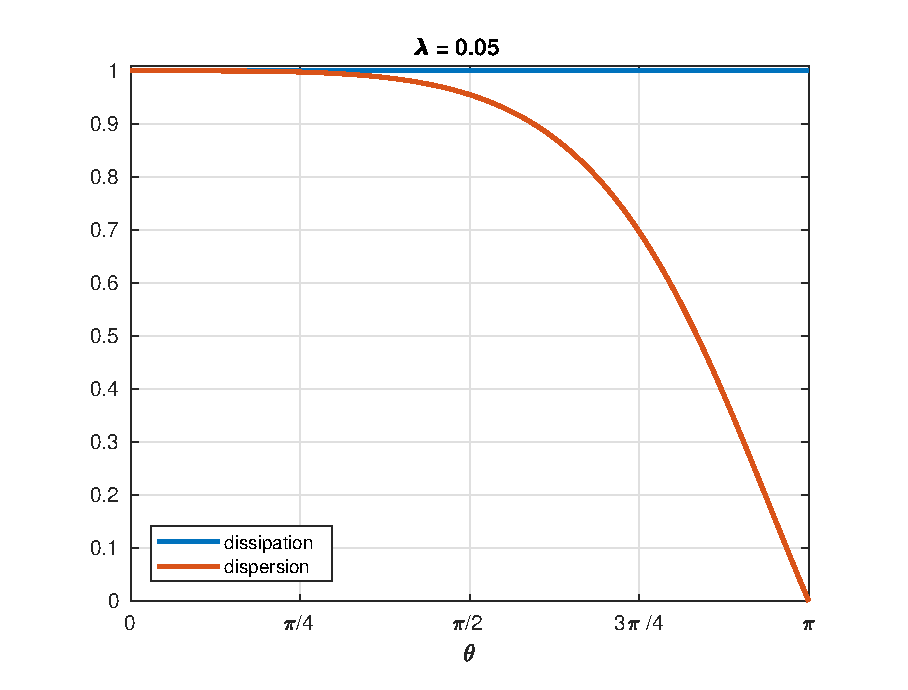
\includegraphics[scale=0.5]{dissip1.eps}
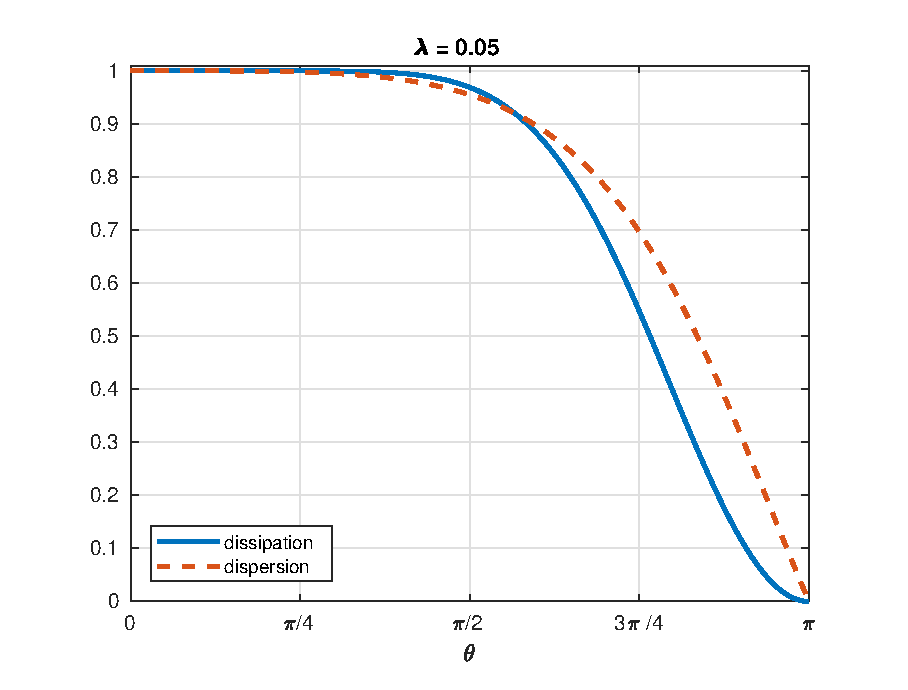
\includegraphics[scale=0.5]{dissipf1.eps}\\
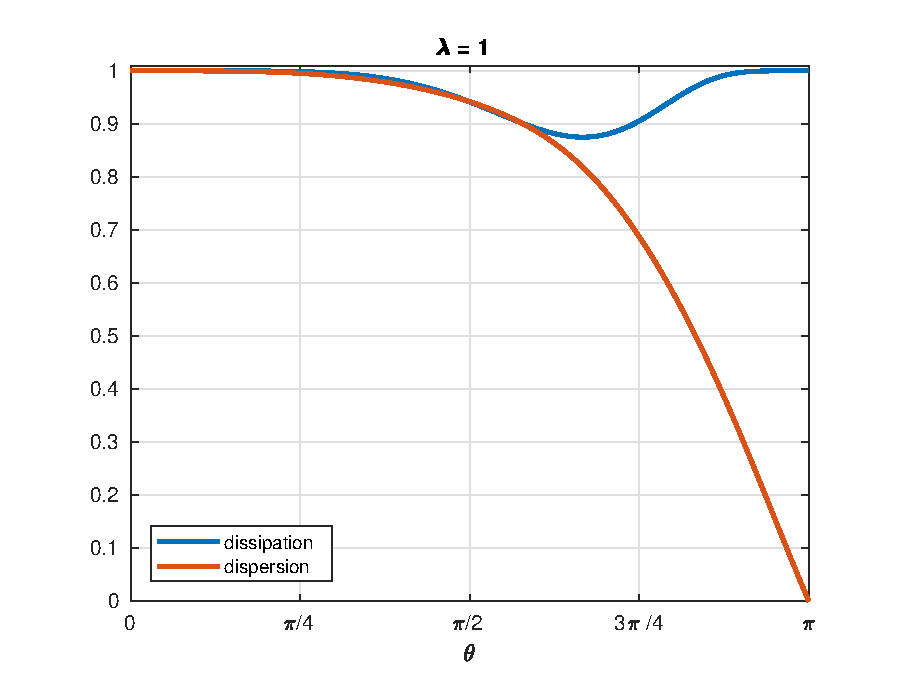
\includegraphics[scale=0.5]{dissip2.eps}
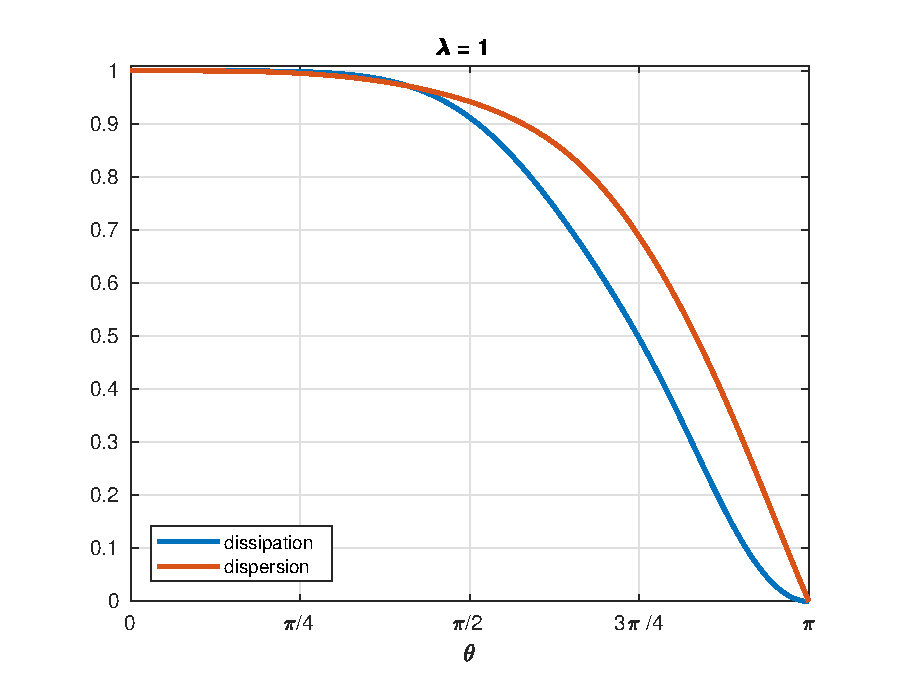
\includegraphics[scale=0.5]{dissipf2.eps}\\
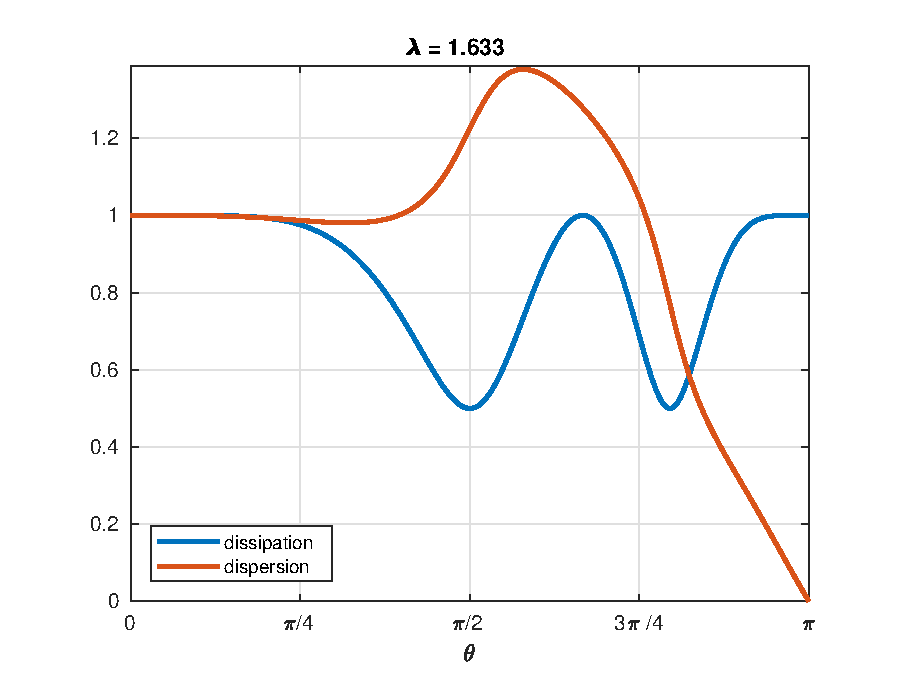
\includegraphics[scale=0.5]{dissip3.eps}
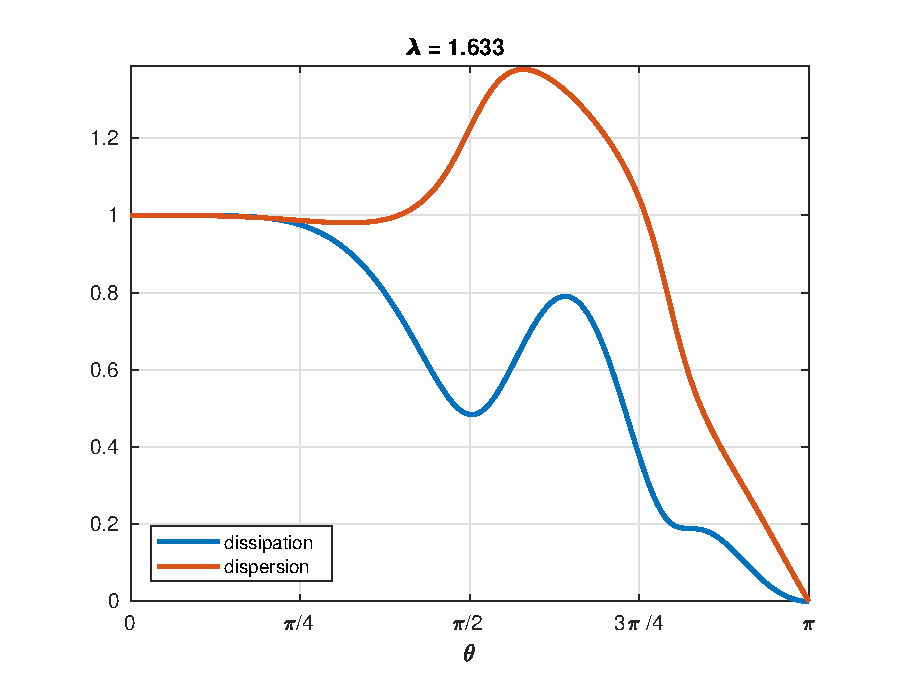
\includegraphics[scale=0.5]{dissipf3.eps}\\
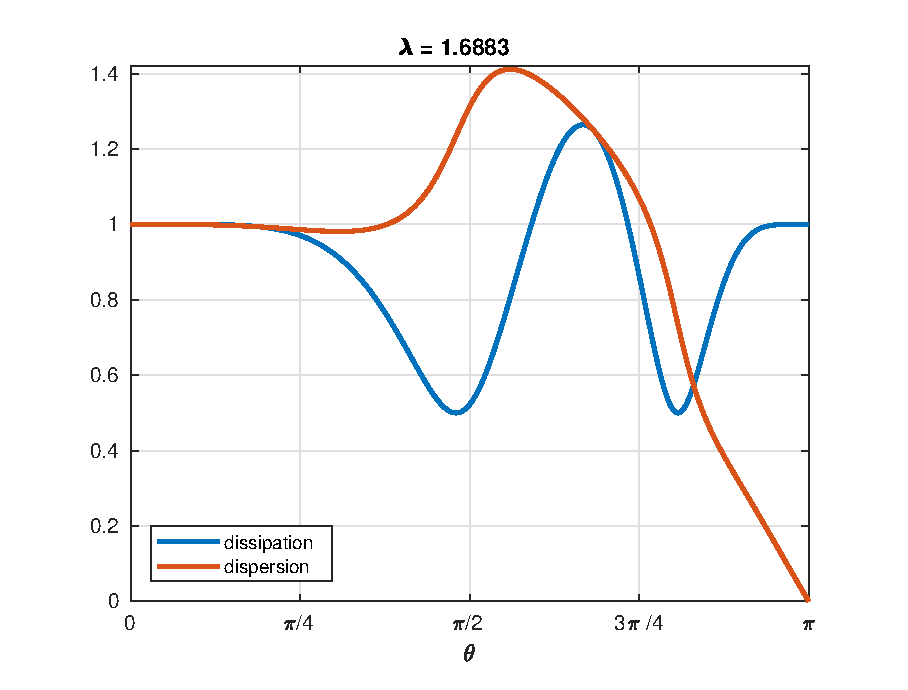
\includegraphics[scale=0.5]{dissip4.eps}
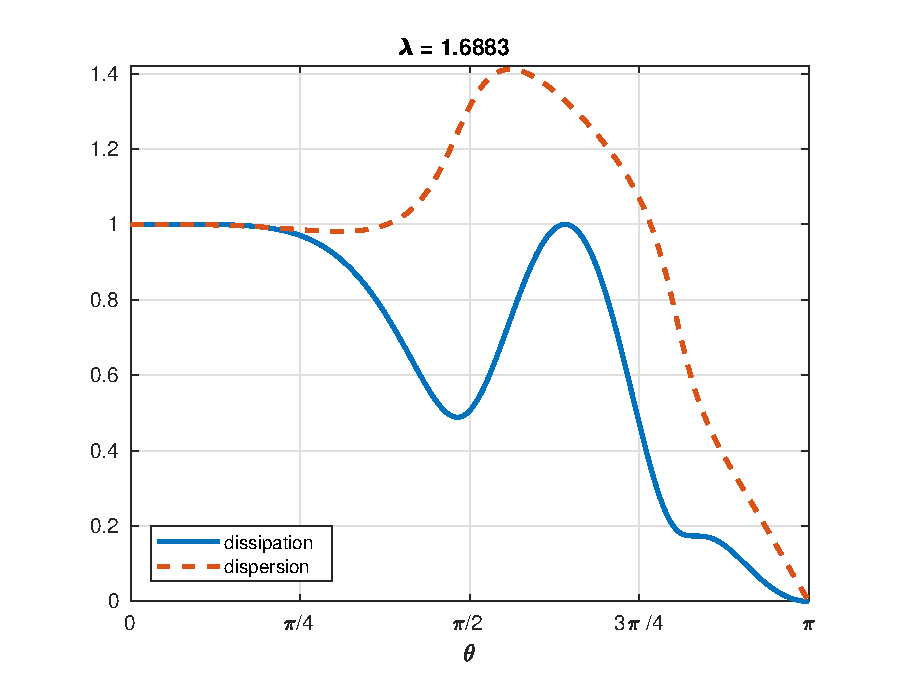
\includegraphics[scale=0.5]{dissipf4.eps}
\end{center}
\caption{Fonction de dissipation et de dispersion associée à l'algorithme \ref{alg:RK4_transport1d} de résolution de l'équation \eqref{eq:transport_1D} sans un filtre (gauche) et avec filtre d'ordre 10 (droite) pour différentes valeurs de $\lambda = c \Delta t / h$.}
\label{fig:dissip_disper}
\end{figure}

Dans la figure \ref{fig:dissip_disper}, on représente la fonction de dissipation $\varepsilon_D$ et la fonction de dissipation $\varepsilon_{\Phi}$ pour différentes valeurs de $\lambda$. Le schéma utilisé est celui de Runge-Kutta d'ordre 4 avec un schéma compact d'ordre 4. On compare le résultat sans filtrage et avec le filtrage d'ordre 10. Il s'agit du schéma donné dans l'algorithme \ref{alg:RK4_transport1d}.
On ne trace ces fonctions que pour $\theta \in [0, \pi]$ pour des raisons de parité. Comme attendu le filtrage dissipe les valeurs de $\theta$ prochent de $\pi$. De plus, plus le nombre $\lambda$ est proche de $0$, moins la dissipation des basses valeurs de $\theta$ est importante. 







\subsection{Relations de conservations}

L'équation de transport \eqref{eq:transport_1D} est une équation de conservation. En effet, la proposition suivante est vérifiée :

\begin{proposition}
Si $u$ est une solution périodique de \eqref{eq:transport_1D} alors pour tout $t>0$, on a
\begin{equation}
\gint_0^1 u(x,t)dx = \gint_0^1 u_0(x)dx,
\end{equation}
la "masse" de $u$ est conservée au cours du temps.
\end{proposition}

\begin{proof}
Il suffit de montrer que la quantité
\begin{equation}
\gint_0^1 u(x,t)dx
\end{equation}
est indépendante du temps $t$.

Comme $u$ est solution de \eqref{eq:transport_1D}, on a
\begin{align*}
\dfrac{d}{dt} \gint_0^1 u(x,t) dx & = \gint_0^1 \dfrac{\partial u}{\partial t}(x,t) dx \\
	& = - c \gint_0^1 \dfrac{\partial u}{\partial x} (x,t) dx \\
	& = - c \left[ u(x,t) \right]_{x=0}^{x=1}
	& = 0 \text{ par périodicité de la solution.}
\end{align*}
d'où le résultat souhaité.
\end{proof}

Dans la pratique, la résolution par un schéma numérique peut entraîner une perte de conservation. 
Le schéma utilisé ici dans l'algorithme \ref{alg:RK4_transport1d} est conservatif.

\begin{proposition}
Pour tout $n \in \mathbb{N}$, si $\mathfrak{u}^n$ est calculée par l'algorithme \ref{alg:RK4_transport1d} alors
\begin{equation}
(\mathfrak{u}^{n+1}, \mathfrak{1})_{h,per} = (\mathfrak{u}^n, \mathfrak{1})_{h,per}.
\end{equation}
où $\mathfrak{1}$ est la fonction de grille constante égale à 1.
\end{proposition}

\begin{proof}
Soit $\mathfrak{b} \in l^2_{h,per}$ une fonction de grille quelconque, alors, en notant $b=\vec(\mathfrak{b})$, on a
\begin{align*}
(\delta_{4,x}^H \mathfrak{b}, \mathfrak{1})_{h,per} & = \dfrac{1}{h} \left( Q_4^H(T) b \right) \cdot \mathbf{1}^T \\
	& = \dfrac{1}{h} b \cdot (\bar{Q}_4^H(T) \mathbf{1})^T \\
	& = \dfrac{1}{h} b \cdot \mathbf{0}^T \text{ par antisymétrie de }Q_4^H(T)\\
	& = 0.
\end{align*}
De cette égalité, on peut déduire directement que
\begin{equation}
(K^{(i)}, \mathfrak{1})_{h,per} = 0
\end{equation}
pour tout $i \in \left\lbrace 1, 2, 3, 4 \right\rbrace$.

De là, on déduit :
\begin{align*}
(\mathfrak{u}^{n+1},\mathfrak{1})_{h,per} & =  \left( S(T) \left( U^n + \dfrac{\Delta t}{6}(K^{(1)}+2K^{(2)}+2K^{(3)}+K^{(4)})  \right) \right) \cdot \mathbf{1}^T \\
	& = \left( U^n + \dfrac{\Delta t}{6}(K^{(1)}+2K^{(2)}+2K^{(3)}+K^{(4)})  \right) \cdot \mathbf{1}^T \text{ par symétrie de } S(T)\\
	& = (\mathfrak{u}^n , \mathfrak{1})_{h,per}.
\end{align*}
avec $U^n = \vec_1(\mathfrak{u}^n)$.
\end{proof}

\subsection{Résultats numériques}

Pour évaluer numériquement les performances du schéma numérique, on considère $\Omega=[0,1]$, $c=0.2$ et deux conditions initiales possibles :
\begin{itemize}
\item une condition initiale régulière :
\begin{equation}
u_0(x) = \dfrac{1}{\sqrt{2}} \left[ \cos (2 \pi x) \sin (4 \pi x) + \sin ( 2 \pi x ) \right]
\label{eq:transport1d_test_reg}
\end{equation}
avec $x \in \Omega$,
\item un créneau :
\begin{equation}
u_0(x) = \left\lbrace
\begin{array}{rl}
1 & \text{ si } 0.25 \leq x \leq 0.75 \\
0 & \text{sinon.}
\end{array}
\right.
\label{eq:transport1d_test_ireg}
\end{equation}
\end{itemize}

Pour établir la précision du schéma, on compare la solution exacte en considérant la condition initiale \eqref{eq:transport1d_test_reg} avec la solution numérique associée. L'erreur relative
\begin{equation}
e_l^n = \dfrac{\| \mathfrak{u}^n - u^*(t^n) \|_l}{\| u^*(t^n) \|_l}
\end{equation}
calculée au temps $t^n$ et $l \in \lbrace 2, \infty \rbrace$. Les valeurs obtenues sont données dans la table \ref{tab:transport1d_test_reg}. Les résultats permettent de confirmer la convergence à l'ordre 4 attendue.
\begin{table}[htbp]
\begin{center}
\begin{tabular}{|c||c|c|c|}
\hline
\textbf{N}  & \textbf{norme 2} & \textbf{norme $\infty$} \\
\hline
\hline
$50$   & $1.1158(-2)$  & $1.2630(-2)$  \\
$100$  & $7.1441(-4)$  & $8.0641(-4)$  \\
$500$  & $1.1484(-6)$  & $1.2998(-6)$  \\
$1000$ & $7.1839(-8)$  & $8.1303(-8)$  \\
\hline 
\hline
\textbf{ordre estimé}& $3.9917$ & $3.9913$\\
\hline
\end{tabular}
\end{center}
\caption{Table de convergence de l'algorithme \ref{alg:RK4_transport1d} avec un filtre d'ordre 10 en considérant la condition initiale \eqref{tab:transport1d_test_reg} au temps final $t^n = 10$ et avec $c \Delta t/ h = 1.5$.}
\label{tab:rate_transport1d_test_reg}
\end{table} 
L'erreur est tracée au cours du temps dans la figure \ref{fig:transport1d_test_reg} en normes 2 et infinie.
\begin{figure}[htbp]
\begin{center}
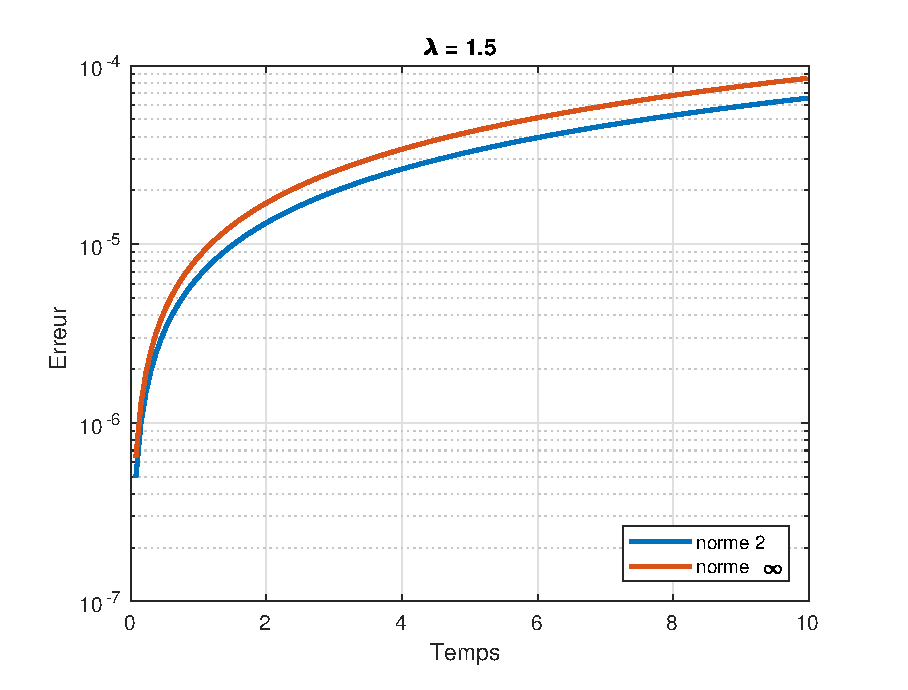
\includegraphics[scale=0.7]{erreurf2_reg.eps}
\end{center}
\caption{Table de convergence de l'algorithme \ref{alg:RK4_transport1d} avec un filtre d'ordre 10 en considérant la condition initiale \label{tab:transport1d_test_reg} au temps final $t^n = 10$, $c \Delta t/ h = 1.6883$ (droite). Le schéma est utilisé avec $N=100$ points de discrétisation.}
\label{fig:transport1d_test_reg}
\end{figure}

La condition initiale \eqref{eq:transport1d_test_reg} est régulière, la solution attendue doit rester régulière. Comme cela est visible dans la figure \ref{fig:comp_ireg}, si l'on utilise la condition initiale \eqref{eq:transport1d_test_ireg}, des oscillations parasites importantes peuvent apparaitre. Il s'agit de phénomènes haute-fréquences qui doivent être atténués par l'utilisation d'un filtre. On compare donc dans la figure \ref{fig:comp_ireg}, la solution au temps $t=10$ obtenue par différentes méthodes de filtrage.
\begin{figure}[htbp]
\begin{center}
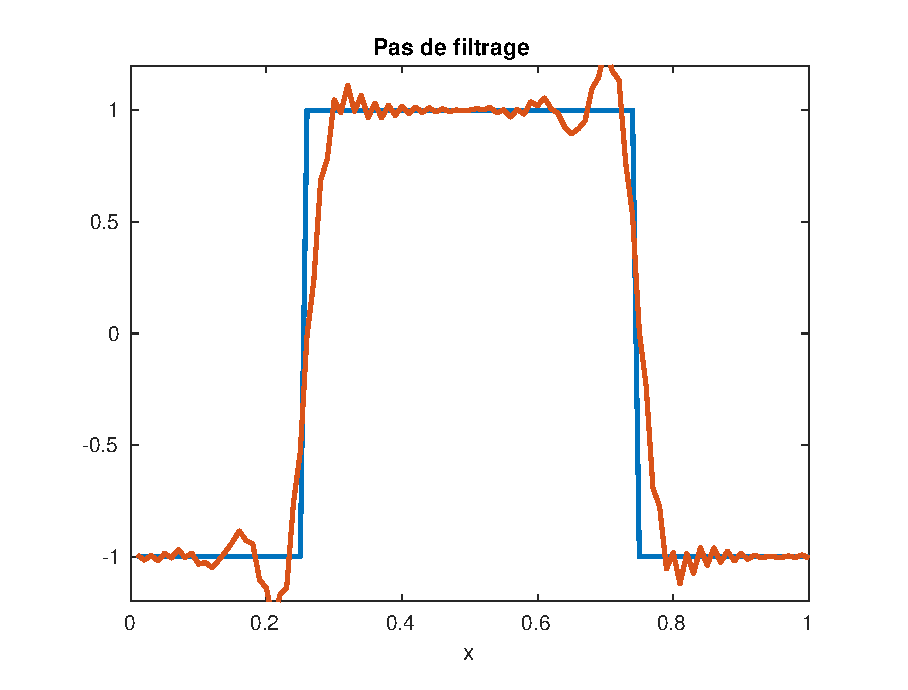
\includegraphics[scale=0.5]{creneau_noftr.eps}
\includegraphics[scale=0.5]{creneau_ftr2.eps}\\
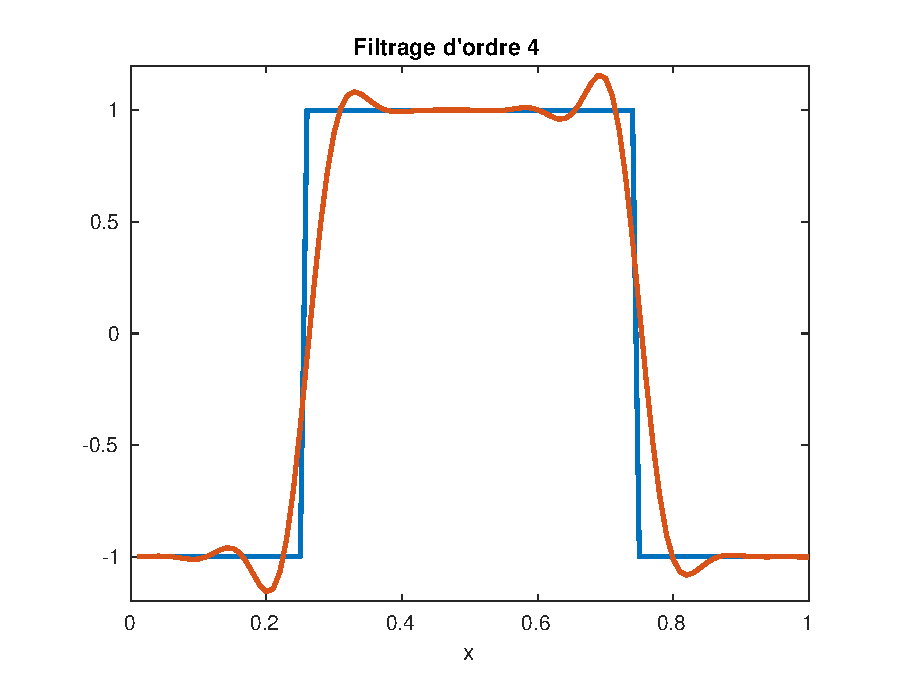
\includegraphics[scale=0.5]{creneau_ftr4.eps}
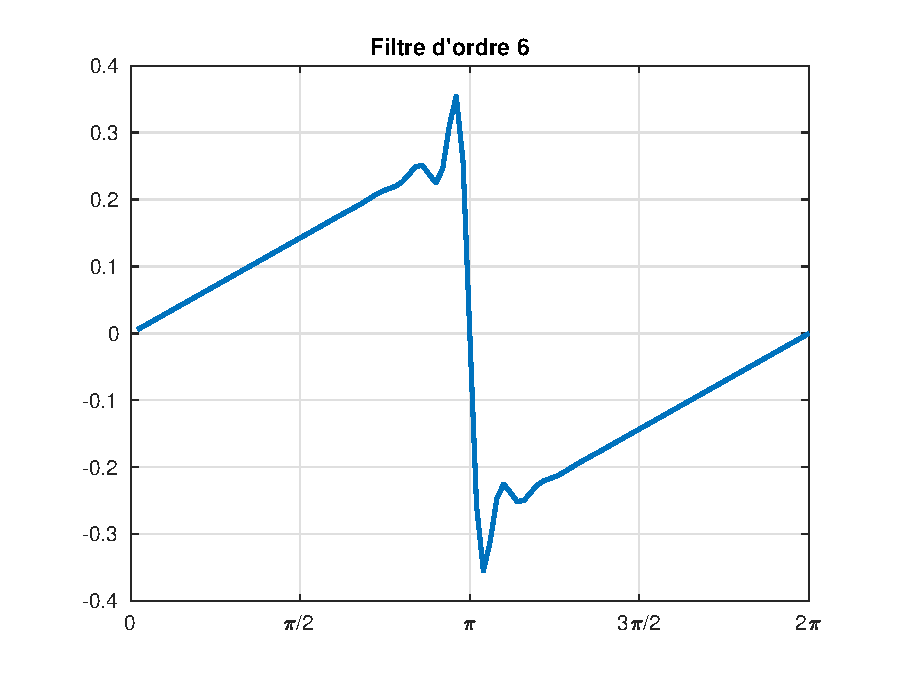
\includegraphics[scale=0.5]{creneau_ftr6.eps}\\
\includegraphics[scale=0.5]{creneau_ftr8.eps}
\includegraphics[scale=0.5]{creneau_ftr10.eps}\\
\end{center}
\caption{Comparaison de la solution exacte (bleu) avec la solution obtenue par l'algorithme \ref{alg:RK4_transport1d} (rouge) au temps $t=10$ pour la résolution de l'équation \eqref{eq:transport_1D} avec différents filtres. $\lambda = c \Delta t / h = 1.5$ et $N=100$.}
\label{fig:comp_ireg}
\end{figure}
On constate dans la figure \ref{fig:comp_ireg} que le filtrage d'ordre 2 permet de supprimer les oscillations parasites mais est beaucoup trop dissipatifs. Les filtres d'ordre 4, 6, 8 et 10 donnent des résultats moins dissipatifs et les oscillations parasites sont atténuées.

















\section{Equation de Burgers en dimension 1}

La solution de l'équation de transport \eqref{eq:transport_1D} ne présente pas d'irrégularités si la solution initiale n'en comporte pas. Cependant lors de la résolution d'équations de conservations non linéaires, des chocs peuvent apparaître, ces solutions sont irrégulières et contiennent des hautes fréquences. On renvoie à \cite{Witham1974} pour plus de détails.

L'exemple le plus simple d'équation de conservation non linéaire est l'équation de Burgers :
\begin{equation}
\dfrac{\partial u}{\partial t} + \dfrac{\partial}{\partial x} \left( \dfrac{u^2}{2}  \right) = 0
\label{eq:burgers_1D}
\end{equation}
pour $x \in [0,L]$, $t>0$ et avec $u(x,t=0)=u_0(x)$. Comme pour l'équation de transport \eqref{eq:transport_1D}, on se place en contexte périodique.

Le schéma numérique utilisé pour résoudre numériquement cette équation est donné par l'algorithme \ref{alg:RK4_burgers1d} où $\mathfrak{u}^n$ est une approximation de $u^*(t^n)$.
\begin{center}
\begin{minipage}[H]{12cm}
  \begin{algorithm}[H]
    \caption{: RK4}\label{alg:RK4_burgers1d}
    \begin{algorithmic}[1]
    \State $\mathfrak{u}^0 = u_0^*$ connu,
    \For{$n=0,1, \ldots$}
             \State  $K^{(1)} = - \dfrac{1}{2}\delta_{4,x}^H \left(\left( \mathfrak{u}^n \right)^2\right)$,
             \State  $K^{(2)} = - \dfrac{1}{2}\delta_{4,x}^H \left(\left( \mathfrak{u}^n + \dfrac{\Delta t}{2} K^{(1)}\right)^2\right)$,
             \State  $K^{(3)} = - \dfrac{1}{2}\delta_{4,x}^H \left(\left( \mathfrak{u}^n + \dfrac{\Delta t}{2} K^{(2)}\right)^2\right)$,
             \State  $K^{(4)} = - \dfrac{1}{2}\delta_{4,x}^H \left(\left( \mathfrak{u}^n + \Delta t K^{(3)}\right)^2\right)$,  
             \State  $\mathfrak{u}^{n+1} = \mathcal{F}\left( \mathfrak{u}^n  + \dfrac{\Delta t}{6} \left( K^{(1)} + 2 K^{(2)} + 2 K^{(3)} + K^{(4)} \right) \right)$.
            \EndFor
    \end{algorithmic}
    \end{algorithm}
\end{minipage}
\end{center}

On peut directement démontrer la proposition suivante :
\begin{proposition}
Pour tout $n \in \mathbb{N}$, si $\mathfrak{u}^n$ est calculée par l'algorithme \ref{alg:RK4_burgers1d} alors
\begin{equation}
(\mathfrak{u}^{n+1}, \mathfrak{1})_{h,per} = (\mathfrak{u}^n, \mathfrak{1})_{h,per}.
\end{equation}
où $\mathfrak{1}$ est la fonction de grille constante égale à 1.
\end{proposition}

L'équation de Burgers \eqref{eq:burgers_1D} est connue pour comporter une discontinuité en temps fini. On choisit $L=1$ et
\begin{equation}
u_0(x) = \sin ( 2 \pi x) \text{ pour tout } x \in [0,L]=[0,1].
\end{equation}

Les résultats sont donnés pour l'algorithme \ref{alg:RK4_burgers1d} sans filtrage dans la figure \ref{fig:comp_burgers}. Des oscillations parasites apparaissent en rendent le calcul très instable. Le schéma numérique ne donne plus de résultats au temps $t=0.4$.
\begin{figure}[htbp]
\begin{center}
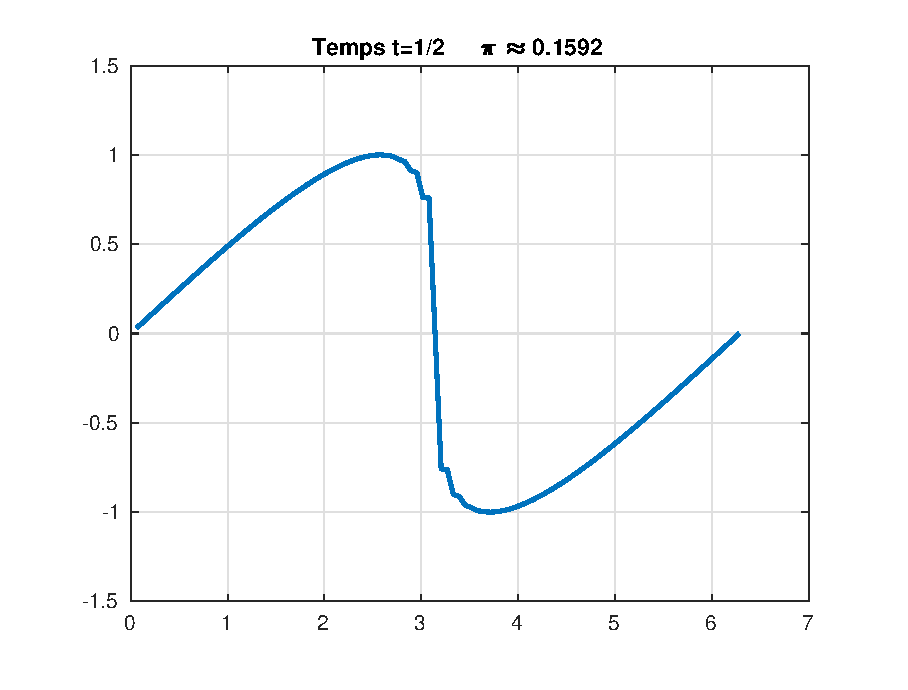
\includegraphics[height=5cm]{burgers_t1.eps}
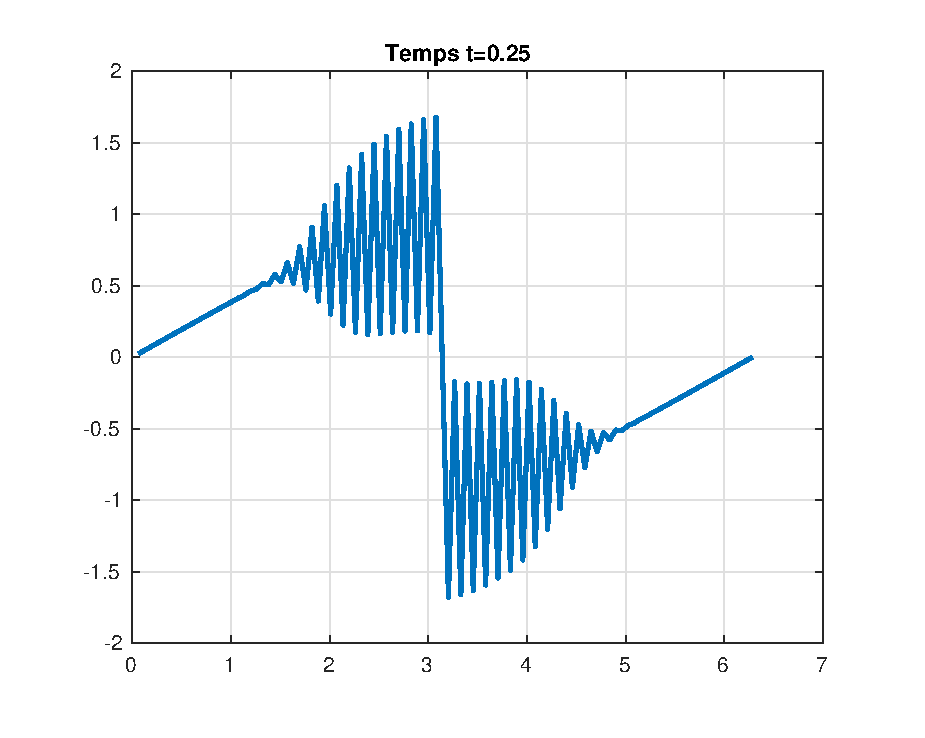
\includegraphics[height=5cm]{burgers_t2.eps}
\end{center}
\caption{Comparaison de la solution numériques obtenue par l'algorithme \ref{alg:RK4_burgers1d} à différents temps pour la résolution de l'équation \eqref{eq:burgers_1D}. On choisit ici $N=100$ et $\Delta t = 10^{-3}$.}
\label{fig:comp_burgers}
\end{figure}

On compare la solution obtenue à l'aide de l'algorithme \ref{alg:RK4_burgers1d} en utilisant différents ordres pour l'opérateur de filtrage. Les résultats sont donnés en figure \ref{fig:comp_burgers_ftr}.
\begin{figure}[htbp]
\begin{center}
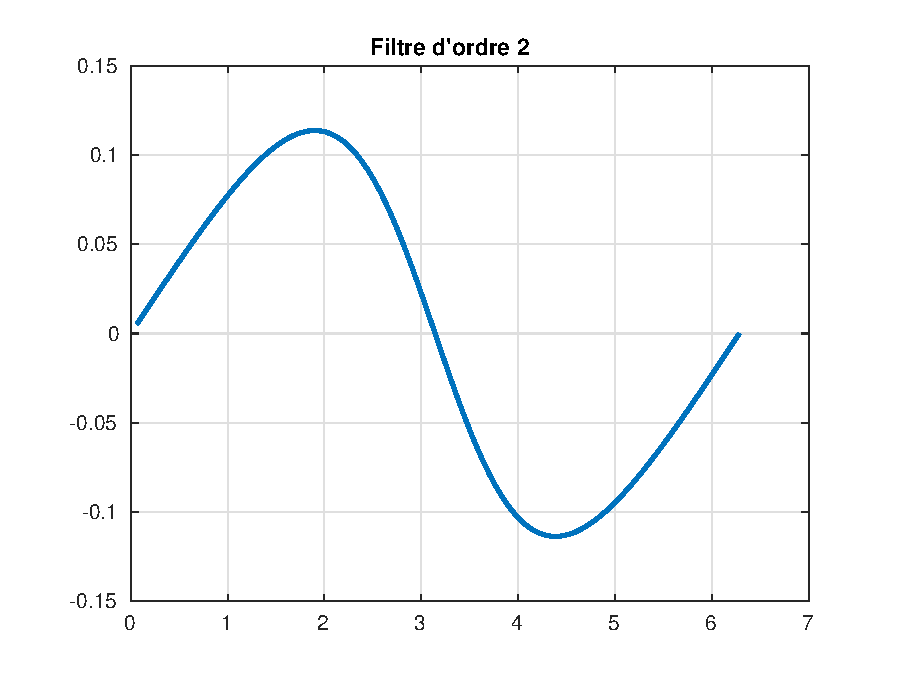
\includegraphics[height=5cm]{burgers_ftr2.eps}
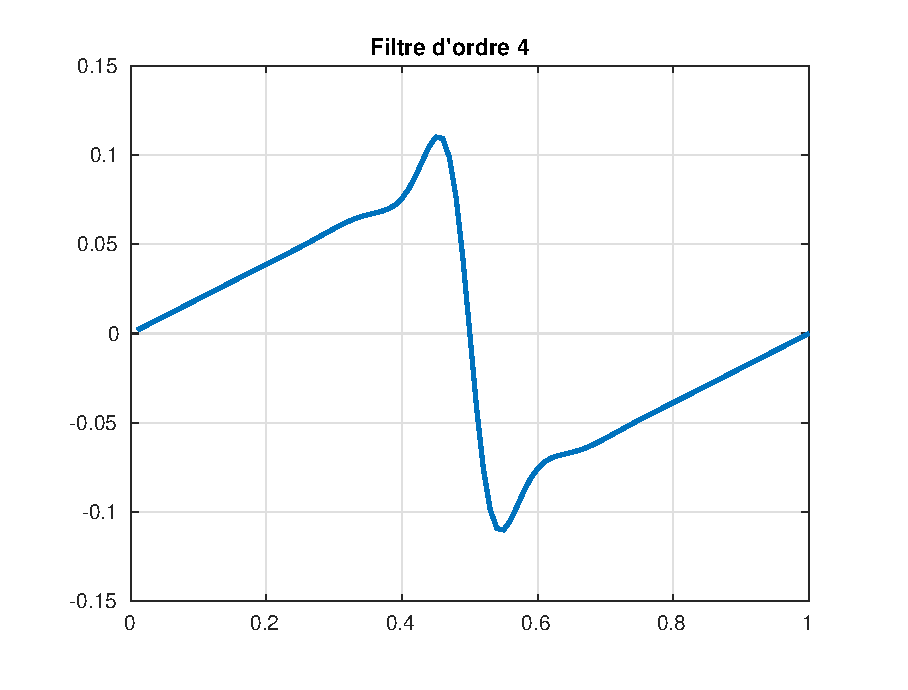
\includegraphics[height=5cm]{burgers_ftr4.eps}\\
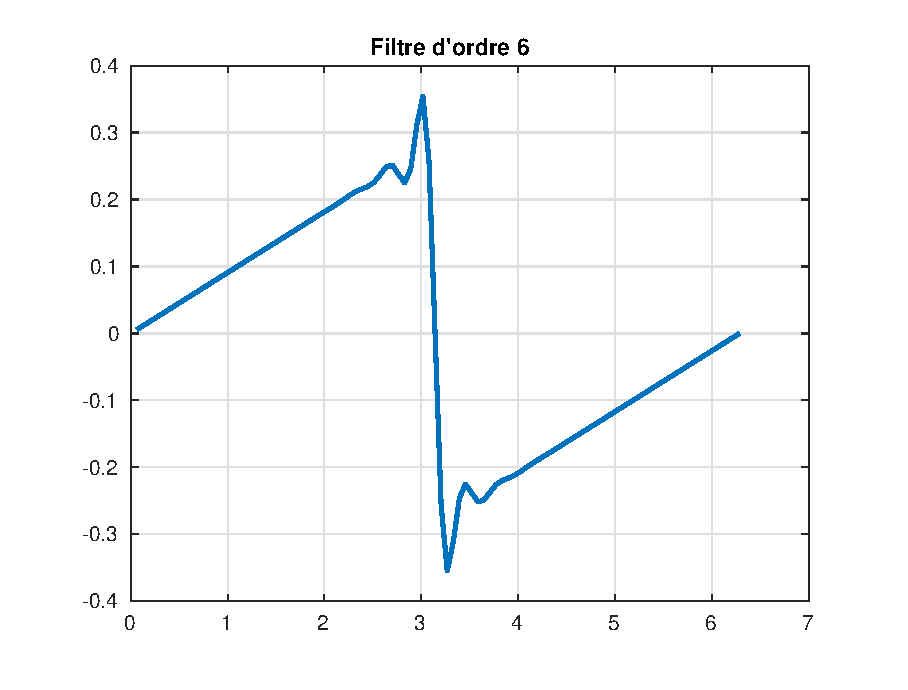
\includegraphics[height=5cm]{burgers_ftr6.eps}
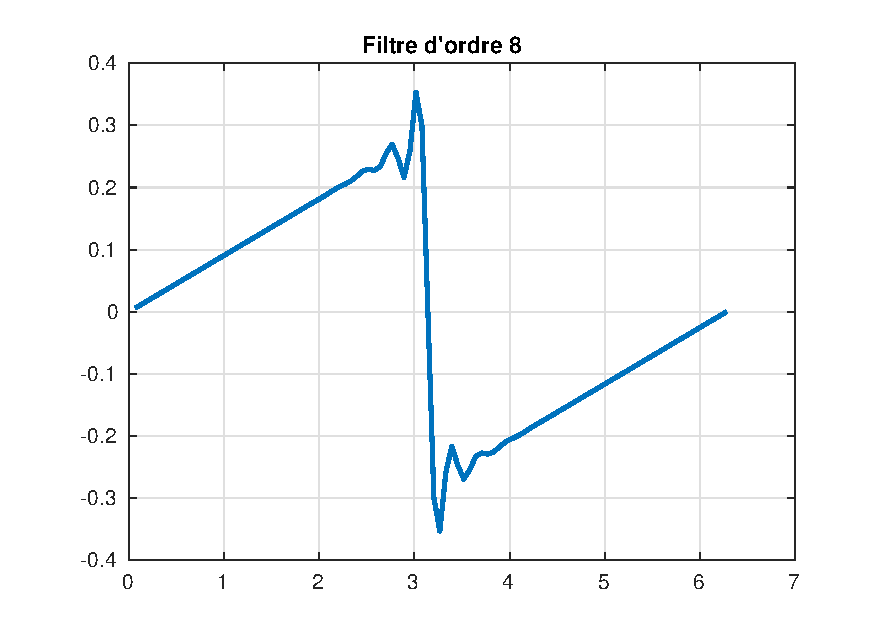
\includegraphics[height=5cm]{burgers_ftr8.eps}\\
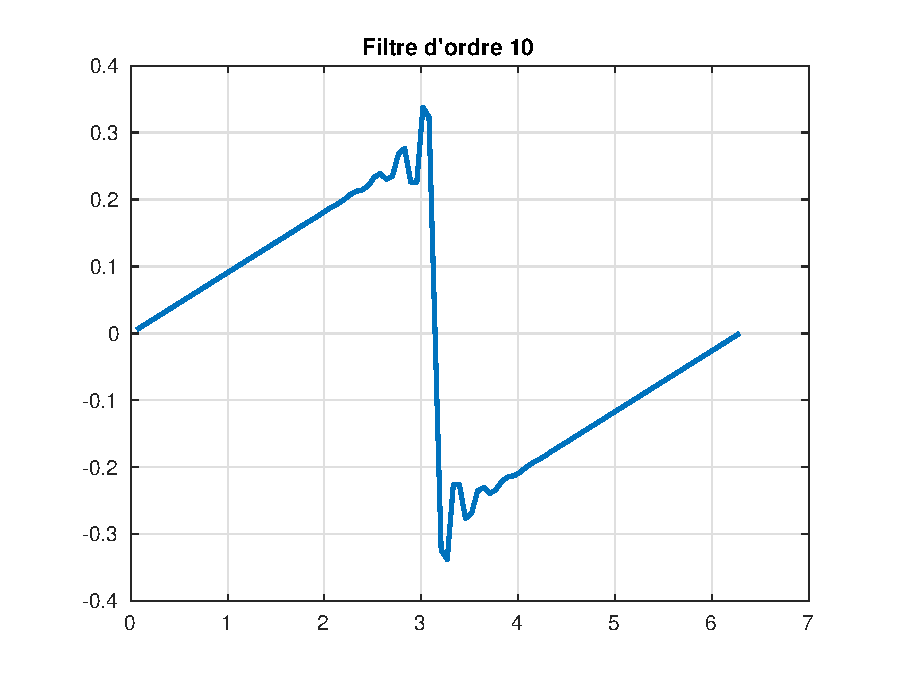
\includegraphics[height=5cm]{burgers_ftr10.eps}
\end{center}
\caption{Comparaison de différentes solution numériques obtenue par l'algorithme \ref{alg:RK4_burgers1d} au temps $t=5$ pour la résolution de l'équation \eqref{eq:burgers_1D} avec différents filtres. On choisit ici $N=100$ et $\Delta t = 10^{-3}$.}
\label{fig:comp_burgers_ftr}
\end{figure}
Le filtrage d'ordre 2 est beaucoup trop dissipatif. Les filtrages d'ordres plus élevés représentent mieux le choc et permettent au schéma de rester stable jusqu'à $t=5$.
















\section{Equation des ondes en dimension 2}

\subsection{Discrétisation}

\subsection{Consistance et Stabilité}

\subsection{Relations de conservations}

\subsection{Résultats numériques}